\subsection{Serie 7}%
\label{sub:serie_7}

\paragraph{Aufgabe 1}%
\label{par:serie_7_aufgabe_1}

Zwei Personen (1 und 2) wählen aus drei Alternativen ($A, B, C$) eine mit Hilfe des
folgenden Verfahrens aus: zuerst streicht Person 1 eine Alternative.
Dann streicht Person 2 eine der verbliebenen Alternativen.
Die dann noch verbliebene Alternative gilt als ausgewählt.
Person 1 zieht die Alternative $A$ der Alternative $B$ vor, die sie wiederum der
Alternative $C$ vorzieht.
Person 2 ordnet die Alternativen gerade umgekehrt.

\begin{enumerate}
  \item Stellen Sie diese Situation durch einen Spielbaum dar.
  \item Bestimmen Sie durch Rückwärtsinduktion das teilspielperfekte Gleichgewicht.
  \item Gibt es andere Nash-Gleichgewichte?
    Gibt es welche, in denen eine andere Alternative als in dem teilspielperfekten
    Gleichgewicht ausgewählt wird?
\end{enumerate}

\subparagraph{Lösung}%

\begin{enumerate}
  \item Es entsteht folgender Spielbaum:
    \begin{center}
      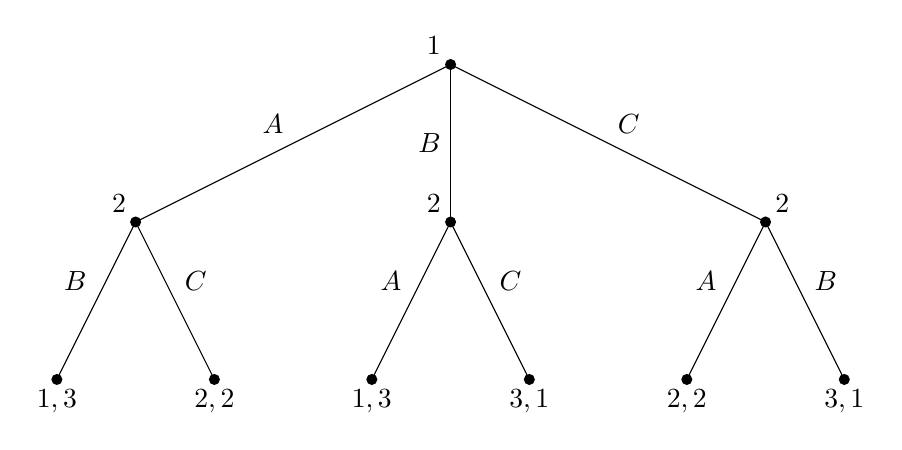
\begin{tikzpicture}
        \fill (0,0) circle (2pt) node [below] {$1,3$};
        \fill (2,0) circle (2pt) node [below] {$2,2$};
        \fill (4,0) circle (2pt) node [below] {$1,3$};
        \fill (6,0) circle (2pt) node [below] {$3,1$};
        \fill (8,0) circle (2pt) node [below] {$2,2$};
        \fill (10,0) circle (2pt) node [below] {$3,1$};

        \fill (1,2) circle (2pt) node [above left] {2};
        \fill (5,2) circle (2pt) node [above left] {2};
        \fill (9,2) circle (2pt) node [above right] {2};

        \fill (5,4) circle (2pt) node [above left] {1};

        \draw (5,4) -- (1,2) node [midway, above left] {$A$};
        \draw (5,4) -- (5,2) node [midway, left] {$B$};
        \draw (5,4) -- (9,2) node [midway, above right] {$C$};

        \draw (1,2) -- (0,0) node [midway, above left] {$B$};
        \draw (1,2) -- (2,0) node [midway, above right] {$C$};
        \draw (5,2) -- (4,0) node [midway, above left] {$A$};
        \draw (5,2) -- (6,0) node [midway, above right] {$C$};
        \draw (9,2) -- (8,0) node [midway, above left] {$A$};
        \draw (9,2) -- (10,0) node [midway, above right] {$B$};
      \end{tikzpicture}
    \end{center}

  \item Es ergeben sich folgende teilspielperfekte Gleichgewichte:
    \begin{center}
      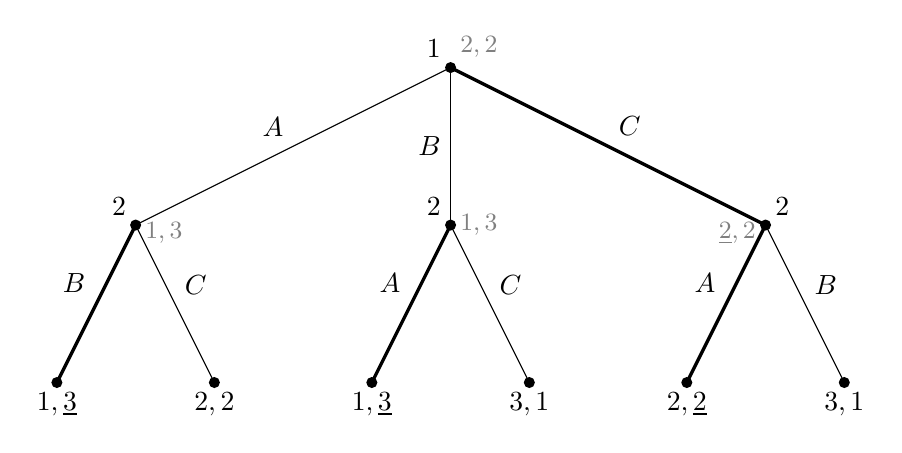
\begin{tikzpicture}
        \fill (0,0) circle (2pt) node [below] {$1,\underline{3}$};
        \fill (2,0) circle (2pt) node [below] {$2,2$};
        \fill (4,0) circle (2pt) node [below] {$1,\underline{3}$};
        \fill (6,0) circle (2pt) node [below] {$3,1$};
        \fill (8,0) circle (2pt) node [below] {$2,\underline{2}$};
        \fill (10,0) circle (2pt) node [below] {$3,1$};

        \fill (1,2) circle (2pt)
          node [above left] {2}
          node [right, yshift=-3pt, gray] {\small $1, 3$};
        \fill (5,2) circle (2pt)
          node [above left] {2}
          node [right, gray] {\small $1, 3$};
        \fill (9,2) circle (2pt)
          node [above right] {2}
          node [left, yshift=-3pt, gray] {\small $\underline{2}, 2$};

        \fill (5,4) circle (2pt)
          node [above left] {1}
          node [above right, gray] {\small $2, 2$};

        \draw (5,4) -- (1,2) node [midway, above left] {$A$};
        \draw (5,4) -- (5,2) node [midway, left] {$B$};
        \draw [very thick] (5,4) -- (9,2) node [midway, above right] {$C$};

        \draw [very thick] (1,2) -- (0,0) node [midway, above left] {$B$};
        \draw (1,2) -- (2,0) node [midway, above right] {$C$};
        \draw [very thick] (5,2) -- (4,0) node [midway, above left] {$A$};
        \draw (5,2) -- (6,0) node [midway, above right] {$C$};
        \draw [very thick] (9,2) -- (8,0) node [midway, above left] {$A$};
        \draw (9,2) -- (10,0) node [midway, above right] {$B$};
      \end{tikzpicture}
    \end{center}
    Damit gilt $\text{SPNE} = \{(C, BAA)\}$.

  \item Wir betrachten alle möglichen Strategien der Spieler:
    \begin{center}
      \begin{tabular}{cccccccccc}
        & & \multicolumn{8}{c}{Spieler 2}\\
        & & $BAA$ & $BAB$ & $BCA$ & $BCB$ & $CAA$ & $CAB$ & $CCA$ & $CCB$\\
        \cmidrule{3-10}
        \multirow{3}{*}{Spieler 1}
        & $A$ & $1,\underline{3}$ & $1,\underline{3}$
              & $1,\underline{3}$ & $1,\underline{3}$
              & $\underline{2},2$ & $2,2$
              & $2,2$ & $2,2$\\
        \cmidrule{3-10}
        & $B$ & $1,\underline{3}$ & $1,\underline{3}$
              & $\underline{3},1$ & $\underline{3},1$
              & $1,\underline{3}$ & $1,\underline{3}$
              & $\underline{3},1$ & $\underline{3},1$\\
        \cmidrule{3-10}
        & $C$ & \framebox{$\underline{2},\underline{2}$} & $\underline{3},1$
              & $2,\underline{2}$ & $\underline{3},1$
              & \framebox{$\underline{2},\underline{2}$} & $\underline{3},1$
              & $2,\underline{2}$ & $\underline{3},1$\\
        \cmidrule{3-10}
      \end{tabular}
    \end{center}
    Damit ist $(C,CAA)$ ein anderes Nash-Gleichgewicht mit reinen Strategien.

    Spieler 2 könnte auch eine gemischte Strategie der beiden Gleichgewichte spielen,
    da Spieler 2 mit jeder Wahrscheinlichkeit $p \in (0,1]$
    für die gemischte Strategie $(C, \langle p \cdot BAA, (1-p) \cdot CAA\rangle)$
    die Auszahlung
    \begin{align*}
      p \cdot 3 + (1-p) \cdot 2 = 2+p
    \end{align*}
    erhält und diese immer echt größer als die Auszahlung der reinen Strategien ist.
\end{enumerate}

\paragraph{Aufgabe 2}%
\label{par:serie_7_aufgabe_2}

Spieler 1 und 2 nehmen an einer Versteigerung teil.
Der Gewinner der Versteigerung erhält $x > 0$ Euro.
Die Regeln sind wie folgt: die Spieler bieten abwechselnd (beginnend mit Spieler 1) bis
entweder ein Spieler passt oder der Betrag von $x-1$ Euro geboten wurde.
Ist ein Spieler am Zug kann er entweder das letzte Gebot um einen Euro überbieten (bei
Beginn des Spiels gilt 0 als das letzte Gebot) oder passen.
\emph{Jeder} Spieler muss \emph{jedes} Gebot, das er macht, umgehend bezahlen
(hat Spieler 1 z.\,B. in einer Partie 1 und 3 (und sonst nichts) geboten, so muss er 4
Euro bezahlen).
Passt Spieler 1 im ersten Zug, so ist Spieler 2 der Gewinner.
Ansonsten ist derjenige Spieler der Gewinner, der das höchste Gebot abgibt.
Die Auszahlung des Gewinners ist $x$ abzüglich der Summe seiner Gebote.
Die Auszahlung des Verlierers ist $0$ abzüglich der Summe seiner Gebote.

\begin{enumerate}
  \item Bestimmen Sie für $x=4$ die teilspielperfekten Gleichgewichte dieses Spiels.
  \item Wiederholen Sie die Aufgabe für $x=5$.
\end{enumerate}

\subparagraph{Lösung}%

\begin{enumerate}
  \item Bei $x=4$ ergibt sich folgender Spielbaum:
    \begin{center}
      \begin{tikzpicture}
        \fill (0,0) circle (2pt) node [above left] {1};

        \fill (-1,-2) circle (2pt) node [above left] {2};
        \fill (1,-2) circle (2pt) node [below] {$0,4$};

        \draw (0,0) -- (-1,-2) node [midway, above left] {$b$};
        \draw (0,0) -- (1,-2) node [midway, above right] {$p$};

        \fill (-2,-4) circle (2pt) node [above left] {1};
        \fill (0,-4) circle (2pt) node [below] {$3,0$};

        \draw (-1,-2) -- (-2,-4) node [midway, above left] {$b$};
        \draw (-1,-2) -- (0,-4) node [midway, above right] {$p$};

        \fill (-3,-6) circle (2pt) node [below] {$0,-2$};
        \fill (-1,-6) circle (2pt) node [below] {$-1,-2$};

        \draw (-2,-4) -- (-3,-6) node [midway, above left] {$b$};
        \draw (-2,-4) -- (-1,-6) node [midway, above right] {$p$};
      \end{tikzpicture}
    \end{center}
    Und folgende teilspielperfekte Gleichgewichte:
    \begin{center}
      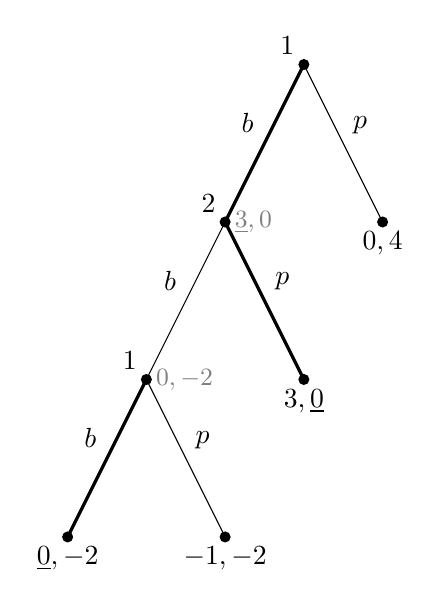
\begin{tikzpicture}
        \fill (0,0) circle (2pt) node [above left] {1};

        \fill (-1,-2) circle (2pt)
          node [above left] {2}
          node [right, gray] {\small $\underline{3},0$};
        \fill (1,-2) circle (2pt) node [below] {$0,4$};

        \draw [very thick] (0,0) -- (-1,-2) node [midway, above left] {$b$};
        \draw (0,0) -- (1,-2) node [midway, above right] {$p$};

        \fill (-2,-4) circle (2pt)
          node [above left] {1}
          node [right, gray] {\small $0,-2$};
        \fill (0,-4) circle (2pt) node [below] {$3,\underline{0}$};

        \draw (-1,-2) -- (-2,-4) node [midway, above left] {$b$};
        \draw [very thick] (-1,-2) -- (0,-4) node [midway, above right] {$p$};

        \fill (-3,-6) circle (2pt) node [below] {$\underline{0},-2$};
        \fill (-1,-6) circle (2pt) node [below] {$-1,-2$};

        \draw [very thick] (-2,-4) -- (-3,-6) node [midway, above left] {$b$};
        \draw (-2,-4) -- (-1,-6) node [midway, above right] {$p$};
      \end{tikzpicture}
    \end{center}
    Es gilt $\text{SPNE} = \{(bb,p)\}$.

  \item $x=5$:
    \begin{center}
      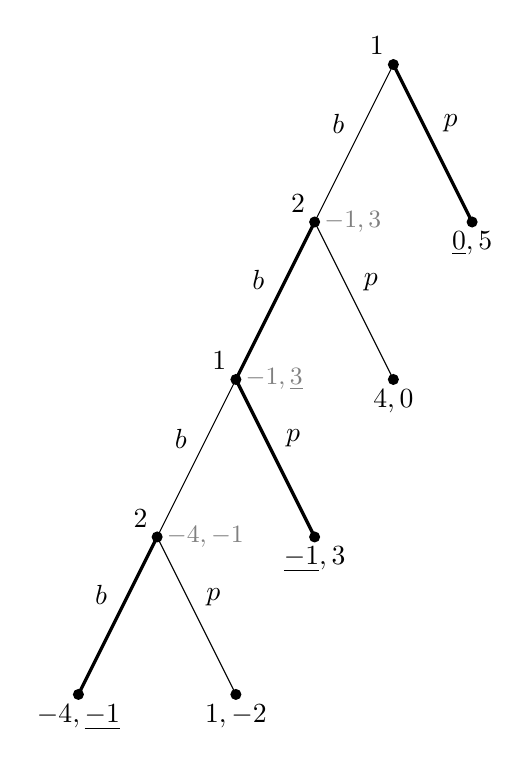
\begin{tikzpicture}
        \fill (0,0) circle (2pt) node [above left] {1};

        \fill (-1,-2) circle (2pt)
          node [above left] {2}
          node [right, gray] {\small $-1,3$};
        \fill (1,-2) circle (2pt) node [below] {$\underline{0},5$};

        \draw (0,0) -- (-1,-2) node [midway, above left] {$b$};
        \draw [very thick] (0,0) -- (1,-2) node [midway, above right] {$p$};

        \fill (-2,-4) circle (2pt)
          node [above left] {1}
          node [right, gray] {\small $-1,\underline{3}$};
        \fill (0,-4) circle (2pt) node [below] {$4,0$};

        \draw [very thick] (-1,-2) -- (-2,-4) node [midway, above left] {$b$};
        \draw (-1,-2) -- (0,-4) node [midway, above right] {$p$};

        \fill (-3,-6) circle (2pt)
          node [above left] {2}
          node [right, gray] {\small $-4,-1$};
        \fill (-1,-6) circle (2pt) node [below] {$\underline{-1},3$};

        \draw (-2,-4) -- (-3,-6) node [midway, above left] {$b$};
        \draw [very thick] (-2,-4) -- (-1,-6) node [midway, above right] {$p$};

        \fill (-4,-8) circle (2pt) node [below] {$-4,\underline{-1}$};
        \fill (-2,-8) circle (2pt) node [below] {$1,-2$};

        \draw [very thick] (-3,-6) -- (-4,-8) node [midway, above left] {$b$};
        \draw (-3,-6) -- (-2,-8) node [midway, above right] {$p$};
      \end{tikzpicture}
    \end{center}
    Daraus folgt $\text{SPNE} = \{(pp,bb)\}$.
\end{enumerate}

\paragraph{Aufgabe 3}%
\label{par:serie_7_aufgabe_3}

Nehmen Sie an, dass in einer Variante des Spiels \emph{Bach oder Strawinski}
\begin{center}
  \begin{tabular}{cccc}
    & & \multicolumn{2}{c}{Spieler 2}\\
    & & $B$ & $S$\\
    \cmidrule{3-4}
    \multirow{2}{*}{Spieler 1}
    & $B$ & $2,1$ & $0,0$\\
    \cmidrule{3-4}
    & $S$ & $0,0$ & $1,2$\\
    \cmidrule{3-4}
  \end{tabular}
\end{center}
die Spieler ihre Aktionen nicht gleichzeitig sondern hintereinander wählen (Spieler 1 ist
zuerst am Zug, Spieler 2 kann die Aktion von Spieler 1 beobachten, bevor er seine Aktion
wählt).
\begin{enumerate}
  \item Bestimmen Sie die strategische Form dieses Spiels.
  \item Bestimmen Sie die Nash-Gleichgewichte in reinen Strategien.
  \item Welches dieser NGG ist teilspielperfekt?
\end{enumerate}

\subparagraph{Lösung}%
\begin{enumerate}
  \item Das Spiel hat folgende strategische Form:
    \begin{center}
      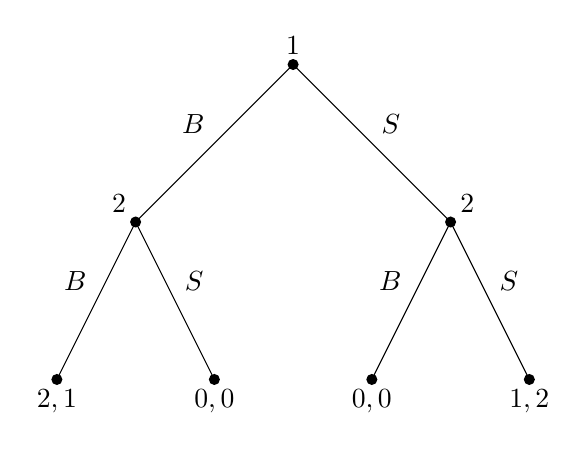
\begin{tikzpicture}
        \fill (0,0) circle (2pt) node [above] {1};

        \fill (-2,-2) circle (2pt) node [above left] {2};
        \fill (2,-2) circle (2pt) node [above right] {2};

        \draw (0,0) -- (-2,-2) node [midway, above left] {$B$};
        \draw (0,0) -- (2,-2) node [midway, above right] {$S$};

        \fill (-3,-4) circle (2pt) node [below] {$2,1$};
        \fill (-1,-4) circle (2pt) node [below] {$0,0$};
        \fill (1,-4) circle (2pt) node [below] {$0,0$};
        \fill (3,-4) circle (2pt) node [below] {$1,2$};

        \draw (-2,-2) -- (-3,-4) node [midway, above left] {$B$};
        \draw (-2,-2) -- (-1,-4) node [midway, above right] {$S$};
        \draw (2,-2) -- (1,-4) node [midway, above left] {$B$};
        \draw (2,-2) -- (3,-4) node [midway, above right] {$S$};
      \end{tikzpicture}
    \end{center}

  \item Zur Bestimmung der Nash-Gleichgewichte betrachten wir alle möglichen Strategien
    der Spieler:
    \begin{center}
      \begin{tabular}{cccccc}
        & & \multicolumn{4}{c}{Spieler 2}\\
        & & $BB$ & $BS$ & $SB$ & $SS$\\
        \cmidrule{3-6}
        \multirow{2}{*}{Spieler 1}
        & $B$ & $\underline{2},\underline{1}$ & $\underline{2},\underline{1}$
              & $0,0$ & $0,0$\\
        \cmidrule{3-6}
        & $S$ & $0,0$ & $1,\underline{2}$ & $0,0$ & $\underline{1},\underline{2}$\\
        \cmidrule{3-6}
      \end{tabular}
    \end{center}
    Damit gilt $\text{NGG} = \{(B,BB), (B,BS), (S, SS)\}$.

  \item Von diesen Gleichgewichten ist nur $(B, BS)$ teilspielperfekt.
\end{enumerate}
